\documentclass{article}
\usepackage[utf8]{inputenc}
\usepackage{amssymb}
\usepackage{amsmath}
\usepackage{mathtools}
\usepackage{graphicx}
\usepackage[export]{adjustbox}

\title{Topics in Design and Analysis of Algorithms\\Problem Set 1}
\author{Adithya Swaroop EE17B115}
\date{March 2021}

\usepackage{natbib}
\usepackage{graphicx}

\begin{document}

\maketitle

\section*{Question 1}
\textbf{(10 points)} Suppose $p_1,...,p_n$ $\in$ [0, 1]$^2$. Let TSP($p_1,...,p_n$) denote the smallest cost of a travelling salesman's tour on $p_1,...,p_n$ with respect to Euclidean distance.  
\begin{enumerate}
    \item (6 points) For any $n > 0$, show that TSP($p_1,...,p_n$) $\leq c\sqrt{n}$ for some constant $c >0$.
    \item (4 points) For any $n > 0$, show that there are $n$ points $q_1,...,q_n$ $\in$ [0, 1]$^2$ such that TSP($q_1,...,q_n$) $\geq c^`\sqrt{n}$ for some constant $c^` >0$.
\end{enumerate}

\subsubsection*{Part 1 solution}
\hspace{8mm} For proving this, let us generate a path of length no more than $k\sqrt{n}$, for some k. Hence TSP($p_1,...,p_n$) is length of smallest tour, it has to be smaller than the path length we generated before.\par
\textbf{Strategy}: We divide unit square into $\sqrt{n}$ strips of equal widths. Then the Salesman uses the following strategy. He begins at leftmost on the topmost strip, and travel right through the line splitting the strip into two halves. If he find a point exactly above or below in the same strip, he travels directly to that point and comes back to centre line of the strip. When he reaches end of square, he travels to middle line of next strip along the edge of the square. Similarly he passes through all strips and finally finishes the loop by coming back to top-left corner.
Now, the total path constitutes of
\begin{itemize}
    \item Length travelled on a strip horizontally
    \item Length travelled on edge vertically
    \item Length travelled from line to point and coming back
    \item Length travelled for closing loop
\end{itemize}
if total length travelled = $d$, 
$$d = \sqrt{n}A+ B+\Sigma C_i+D$$
Also, we know that
$$ A = 1, B \leq 1, C_i \leq 2\frac{1}{2\sqrt{n}}, D \leq \sqrt{2}$$
So, 
$$d \leq \sqrt{n}+ 1+n\frac{1}{\sqrt{n}}+\sqrt{2}$$
$$d \leq 2\sqrt{n}+\sqrt{2}+1$$

As we discussed above, TSP($p_1,...,p_n$) $< d$ and because of that, TSP($p_1,...,p_n$) is also bounded by  $2\sqrt{n}+\sqrt{2}+1$, and it is $O(\sqrt{n})$. So TSP($p_1,...,p_n$) $\leq c\sqrt{n}$ for some constant $c >0$.

\subsection*{Part 2 Solution}
\hspace{8mm}This can be proved if we can find points which gives TSP($q_1,...,q_n$) value which is $\theta(\sqrt{n})$. For that, we use the following strategy. We divide the unit square into n squares, each with side $\frac{1}{\sqrt{n}}$. We can place n points on top-left point of each square. Now, in this case, minimum distance between any two neighbouring points is $\frac{1}{\sqrt{n}}$. As TSP($q_1,...,q_n$) is length of minimum tour covering all points, it has to be greater than $n$ times minimum neighbouring distance.
$$TSP(q_1,...,q_n) \geq n\frac{1}{\sqrt{n}}$$
$$TSP(q_1,...,q_n) \geq \sqrt{n}$$
That's how we can generate points $q_1,...,q_n$ such that we can create lower bound $\theta(\sqrt{n})$ on $TSP(q_1,...,q_n)$. So, TSP($q_1,...,q_n$) $\geq c^`\sqrt{n}$ for some constant $c^` >0$.
\\
\par Above results are valid even if $n$ isn't a perfect square, we can prove the part 1 result by using $n^`$, greatest perfect square less than $n$ and prove part 2 result using $n^`$, least perfect square greater than $n$. Complexity rules are still valid and inequalities can be proved also for $n$.
\newpage
\section*{Question 2}
\textbf{(7 points)} This exercise to demonstrate the limitations of considering expected running
time of an algorithm as a useful measure. For any $n > 0$, describe a function $f : \{0, 1\}^n \rightarrow \mathbb{N} $ such that
\begin{itemize}
    \item $\mathbb{E}[f] = \mathbb{E}_{x \in \{0, 1\}^n}[f(x)] = n^c$ for some constant $c$ and
    \item $var[f] = E[f^2]-(E[f])^2 = \Omega(2^n)$
\end{itemize}
I.e., there can be performance measures $f$ which is polynomial in expectation, but variance being exponential. Give formal justification for your answer (i.e., computation of
expectation and variance for the function $f$ constructed).
\subsection*{Solution 1}
Let function f be like this.  
\[
    f(x) = \max\begin{dcases}
    2^n   &  \mathrm{if}\ x= 1^n \ (11...1)                   \\
    0   &  \mathrm{otherwise}        \\
      \end{dcases}
    \]
\textbf{Expectation:}
$$\mathbb{E}[f] = \frac{1}{2^n}\ 2^n + \frac{2^n-1}{2^n}\ 0$$
$$\mathbb{E}[f] = 1$$
\textbf{Variance:}
$$\mathbb{E}[f^2] = \frac{1}{2^n}\ (2^n)^2 + \frac{2^n-1}{2^n}\ 0$$
$$\mathbb{E}[f^2] = 2^n$$
$$var(f) = \mathbb{E}[f^2] - (\mathbb{E}[f])^2$$
$$var(f) = 2^n - 1$$
$$var(f) = \Omega(2^n)$$
Expectation of running time of an algorithm as a performance measure is not always suggested. Because of high variance, sometimes, it takes forever for program to finish. A good performance measure has not only good expected value but also a good variance.
\subsection*{Solution 2}
Another example of $f(x)$ can be this.
$$f(x) = 2(2^nx_1-2^nx_2+x_3+x_4+..+x_n)+2$$
\textbf{Expectation:}
$$\mathbb{E}[f] = 2(2^n\mathbb{E}[x_1]-2^n\mathbb{E}[x_2]+\mathbb{E}[x_3]+\mathbb{E}[x_4]+..+\mathbb{E}[x_n])+2$$
$$\mathbb{E}[x_i] = 0.5, \ var[x_i] = 0.25$$
$$\mathbb{E}[f] = 2(2^n\frac{1}{2}-2^n\frac{1}{2}+\frac{1}{2}+\frac{1}{2}+..+\frac{1}{2})+2$$
$$\mathbb{E}[f] = 2(\frac{n-2}{2})+2$$
$$\mathbb{E}[f] = n$$
\textbf{Variance:}\\
as $var(aX+bY+c) = a^2var(X)+ b^2var(Y)$,
$$var(f) = 2^2(2^{2n}var(x_1)+2^{2n}var(x_2)+var(x_3)+var(x_4)+..+var(x_n))$$
$$var(f) = 4 \ (2^{2n} \ \frac{1}{4}+2^{2n} \ \frac{1}{4}+\frac{1}{4}+\frac{1}{4}+..+\frac{1}{4})$$
$$var(f) = (2^{2n}+2^{2n}+1+1+..+1)$$
$$var(f) = n-2+2^{2n+1}$$
$$var(f) = \Omega(2^{2n})$$

\newpage
\section*{Question 3}
\textbf{(7 points)} Obtain profits $p_1,...,p_n$ and weights $w_1,...,w_n$ for the knapsack problem so that $|\mathcal{P}|$ is exponential in n (e.g $2^{\Omega(n)}$). Justify your answer.
\subsection*{Solution}
\hspace{5mm}Total number of possible combinations of items possible are exponential($2^n$). So, for making cardinality of pareto-optimal set exponential, we can make every possible combination (every possible $x$) a pareto-optimal solution and $|\mathcal{P}| = 2^n$.

So, for making every $x$ pareto-optimal, we should make sure that any $y \in \mathcal{S}$ doesn't dominate any other $x\in \mathcal{S}$. By \textit{dominate}, we mean that $y$ having more total profit but less total weight compared to $x$. 
\par Graphically, if we plot $(p_i, w_i)$ for  $x_i$'s, a point is said to be pareto-optimal, if there are no other points to the left-top part of that point. Now, for making every point pareto-optimal we can line-up every point on a same line, $p = mw$ for example, $m$ is slope of the line. This works because, now for any point, there is no other point top-left to it.
\par \textbf{So, we can generate $w_i$'s and then generate $p_i = m w_i$ for every $1\leq i\leq n$ for any integer $m$.} Now, any linear combination of $(p_i, w_i)$'s will also be on the same line, As all possible points lie on the same line, all are pareto-optimal. \\ \\
\textbf{Proof:} Suppose $x \in \{0, 1\}^n$ denoting whether an object is present or not. $p$, $w$ are vectors containing all profits and all weights respectively and $p=mw$ according to our assumption. Let's prove that no other $y \in \{0, 1\}^n$ dominates x by contradiction.
\par Suppose $y$ dominates x.
$$p_y \geq p_x, w_y \leq w_x, \text{one of the inequalities is strict.}$$
$$p = mw, p_y = p^Ty, w_y = w^Tx$$
$$\text{if }p_y \geq p_x \Rightarrow mw_y \geq mw_x$$
$$w_y \geq w_x \  \text{(contradiction)}$$
$$\text{if }w_y \leq w_x \Rightarrow \frac{p_y}{m} \leq \frac{p_x}{m}$$
$$p_y \leq p_x \ \text{(contradiction)}$$
It is a contradiction to our assumption. No possible solution dominates any other solution, so all $x \in \mathcal{S}$ belongs to pareto-optimal set. $|\mathcal{P}| = 2^n$.
\newpage
\section*{Question 4}
\textbf{(6 points)} Read the proof of Lemma 3.4 in the notes by Bodo Manthey (in the google drive shared with the class). The proof assumes that $a = (0,...,0)$ and $b = (\delta,...,0)$.
Why is this assumption without loss of generality? Justify your answer.
\subsection*{Solution}
Bi-variate Gaussian Distribution is rotationally symmetric. If $X$ and $Y$ have independent unit normal distributions then their joint
distribution $f(x, y)$ is given by
$$f(x, y) = \phi(x)\phi(y) = c^2e^{-\frac{1}{2}(x^2+y^2)}$$
Now, even if axes are rotated to $(X^`, Y^`)$, still $x^{`2}+y^{`2} = x^2+y^2$ , joint distribution doesn't change. (as $x^{`2}+y^{`2}$ is still the same squared distance from origin) Therefore it is rotationally symmetric.\par
\begin{figure}[h!]
    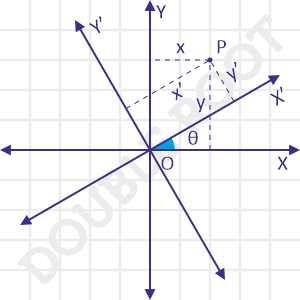
\includegraphics[width=0.4\textwidth, center ]{image.png}
\end{figure}
\textbf{Also we are not concerned about the values of Gaussian distribution, rather we are concerned about how Gaussian distribution \textit{variates}.} So, we can change the origin to one of the point and change the axes such that one axis is line joining two points, without loss of any generality and it's now easier for us to compute.\\
Now, we can assume $c=(c_1, c_2)$ in the new axes which are both translated and rotated.
$$a=(0,0), b=(\delta,0), ||a-b||_2 = \delta$$

\end{document}
